\subsection{Kurvengetriebe (CAM-Mechanism) \hfill IP}
\begin{footnotesize}
    \begin{center}
        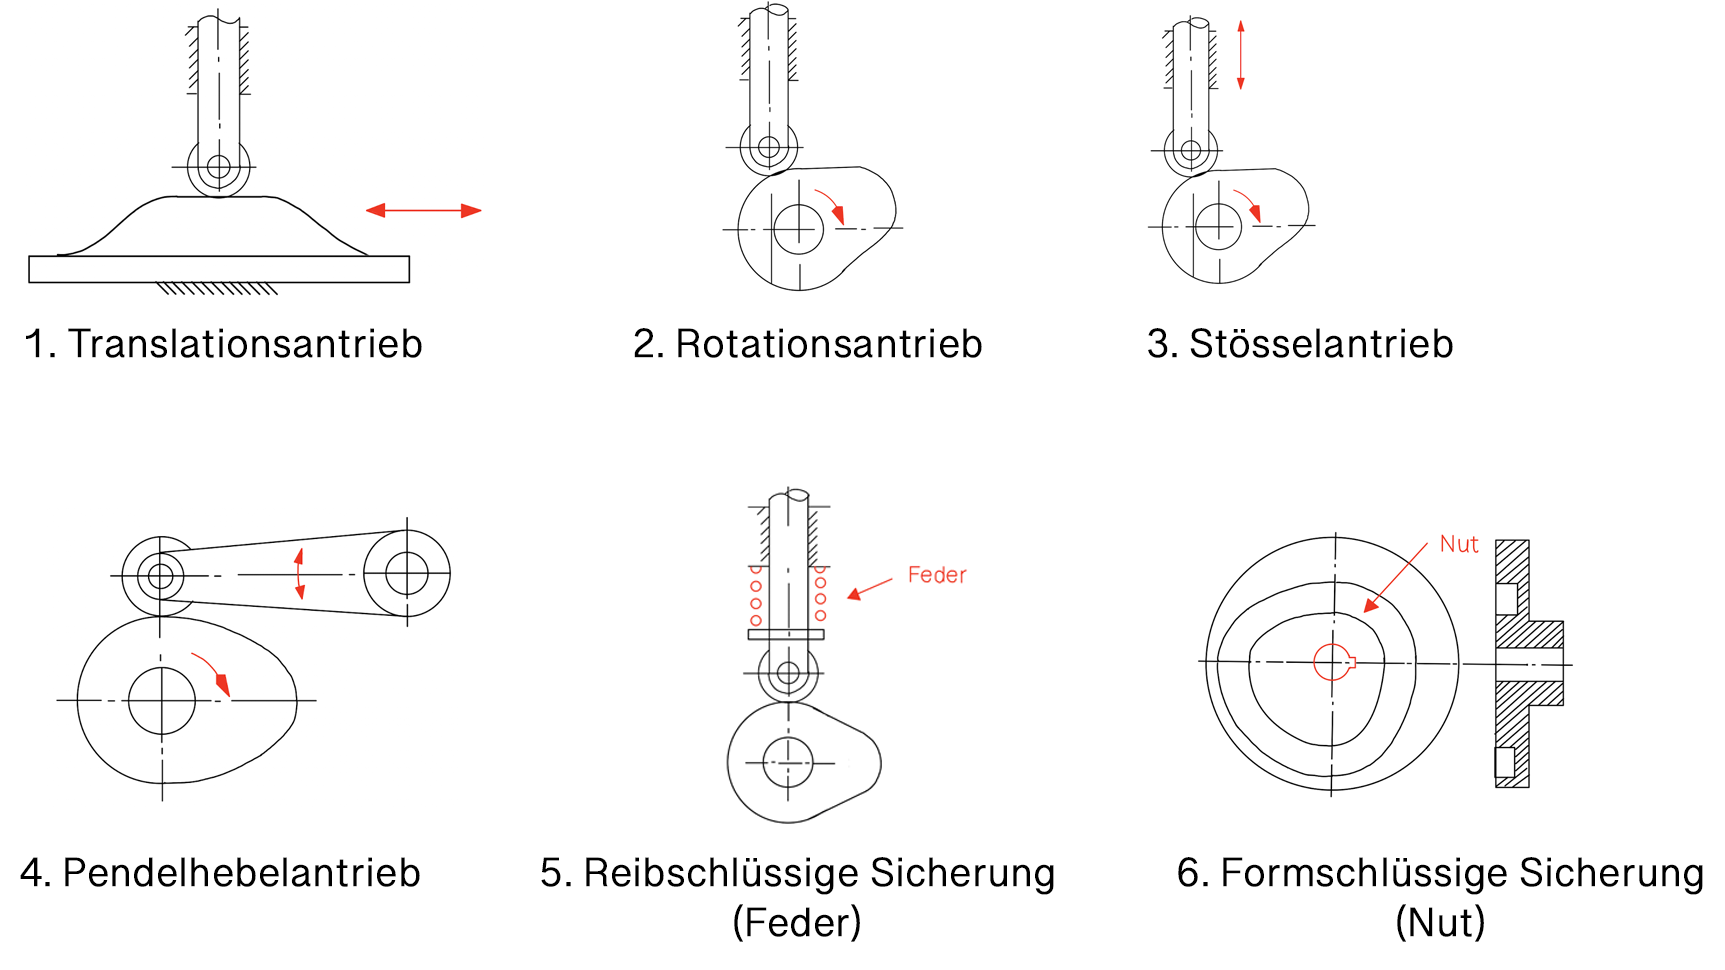
\includegraphics[width = 0.8\linewidth]{src/images/MAEIP_Kurvengetriebe}
        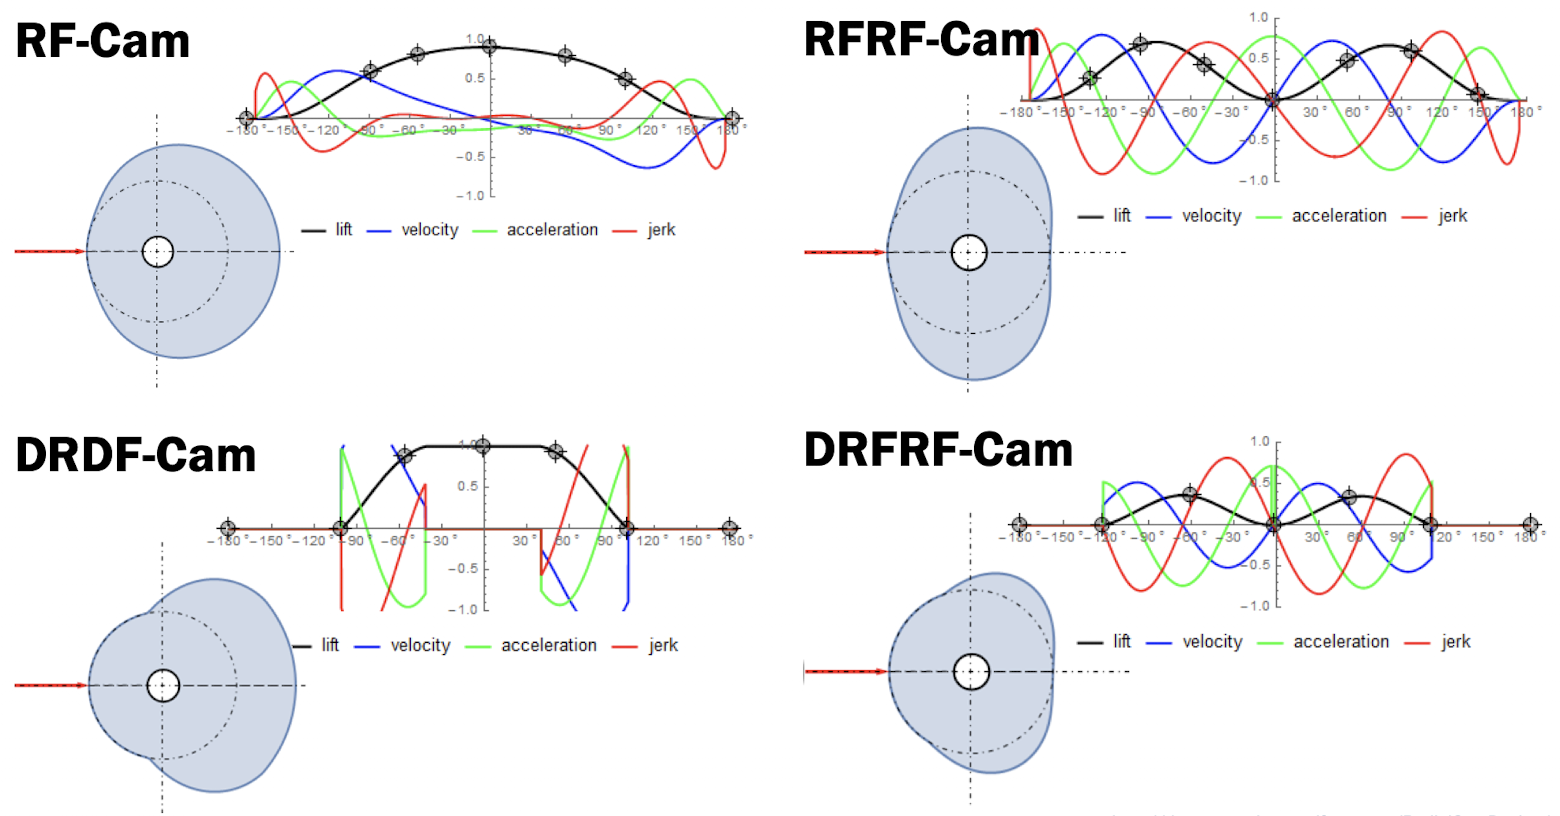
\includegraphics[width = 0.75\linewidth]{src/images/MAEIP_VariationKurvenform}
        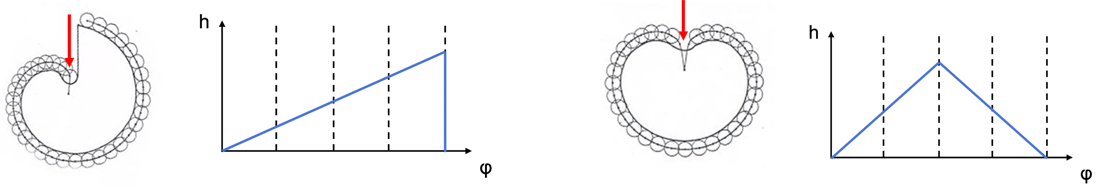
\includegraphics[width = 0.8\linewidth]{src/images/MAEIP_ArchimedesKurvenform}
    \end{center}
    \begin{itemize}
        \item \textbf{Formen Kurvengetriebe:} 
        \\ R = Rise $\quad \mid \quad$ F = Fall $\quad \mid \quad$ D = Dwell
        \item \textbf{Legende Cam-Diagramme:}
        \\ \colorbox{Black}{\color{white} Lift} \colorbox{Cyan}{Velocity} \colorbox{LimeGreen}{Acceleration} \colorbox{Red}{Jerk}
    \end{itemize}
\end{footnotesize}